\def\year{2020}\relax

\documentclass[letterpaper]{article}

\usepackage{aaai20}
\usepackage{times}
\usepackage{helvet}
\usepackage{courier}
\usepackage[hyphens]{url}
\usepackage{graphicx}
\urlstyle{rm}
\def\UrlFont{\rm}

\usepackage{graphicx}
\frenchspacing
\setlength{\pdfpagewidth}{8.5in}
\setlength{\pdfpageheight}{11in}

\usepackage{amsmath,amssymb,amsthm}
\usepackage[vlined,algoruled,titlenumbered,noend,portugues]{algorithm2e}
\usepackage{booktabs}

\graphicspath{{./images/}}

\pdfinfo{
  /Title (Relatório 01 - Algoritmos de Planejamento Probabilístico)
  /Author (Daniel Baptista Dias)
}

% /Title (Relatório 01 - Algoritmos de Planejamento Probabilístico)
% /Author (Daniel Baptista Dias)

\setcounter{secnumdepth}{0} %May be changed to 1 or 2 if section numbers are desired.

% The file aaai20.sty is the style file for AAAI Press proceedings, working notes, and technical reports.
\setlength\titlebox{2.5in} % If your paper contains an overfull \vbox too high warning at the beginning of the document, use this
% command to correct it. You may not alter the value below 2.5 in

\title{Relatório 01 - Algoritmos de Planejamento Probabilístico}
\author{Daniel Baptista Dias}

\begin{document}

\maketitle

\section{Introdução}
\label{sec:introducao}

Na disciplina de Inteligência Artificial existe uma área chamada de Planejamento Automatizado
que estuda formas de como um agente pode tomar um conjunto de decisões em sequência interagindo
com um ambiente com o objetivo de solucionar um problema.

O foco deste trabalho será em uma das subáreas do Planejamento Automatizado, o Planejamento Probabilístico, onde
é assumido que o resultado da interação do agente com o ambiente é incerto, e que dada uma ação realizada pelo agente
em um ambiente dada uma determinada situação, essa ação pode ter diferentes resultados, cuja frequência é ditada por
uma distribuição de probabilidades.

Um arcabouço utilizado para modelar problemas de Planejamento Probabilístico é utilizar os Processos Markovianos de Decisão
(MDP, do inglês \textit{Markov Decision Processes})\cite{Puterman-1994} que possui alguns algoritmos conhecidos para resolve-los.

Serão analizados os algoritmos Iteração de Valor \cite{Howard-1960}, RTDP (do inglês, Real Time Dynamic Programming)
\cite{BartoBradtkeSingh-1995} e LRTDP (Labeled Real Time Dynamic Programming) \cite{BonetGeffer-2003} em relação a como eles
solucionam os MDPs.

\section{Arcabouço Teórico}

No contexto de tomada de decisões por um agente em um ambiente completamente observável, um Processo de Decisão Markoviano (MDP)
pode ser descrito por uma tupla $\mathcal{M}=\langle S,A,R,P,\gamma \rangle$, onde:

\begin{itemize}
    \item $S$ é um conjunto de estados finitos e discretos, que definem a situação do ambiente em um determinado momento;
    \item $A$ é um conjunto de ações que o agente pode executar;
    \item $R : S \rightarrow \mathcal{R} $ é a função recompensa, que retorna a recompensa obtida pelo agente ao se alcançar um determinado estado;
    \item $P : S \times A \times S \rightarrow [0, 1]$ é uma função de transição que retorna a probabilidade de um agente, dado que executou uma ação $a \in A$ em um estado $s \in S$, alcançar o estado $s' \in S$. Neste trabalho uma outra notação que também será usada para representar essa transição é $P(s'|s,a)$.
\end{itemize}

Neste ambiente a tomada de decisão ocorre por etapas (estágios), onde o agente executa uma ação de cada vez alterando o estado do ambiente e recebendo uma recompensa ou sendo penalizado com um custo (recompensa negativa). Um problema pode ter três tipos de horizonte, caracterizados pela quantidade de estágios de decisão que o agente poderá tomar:

\begin{itemize}
    \item \textbf{horizonte finito}: o agente tem um número finito de $T$ estágios de decisão;
    \item \textbf{horizonte infinito}: o agente tem infinitos estágios de decisão ($T = \infty$);
    \item \textbf{horizonte indeterminado}: o agente tem possui um número de estágios de decisão desconhecido ($T$ desconhecido).
\end{itemize}

O objetivo do agente neste MDP é encontrar uma política $\pi : S \rightarrow A$ que indique a melhor ação a ser tomada em cada estado $s$ a fim de se obter a maior recompensa possível.

Para identificar esta política pode-se calcular o valor dela para cada estado $s$ através do critério da recompensa esperada total. Esse critério indica o quanto de recompensa um agente pode receber em média a executar uma política $\pi$ a partir do estado $s_0 = s$ até o instante $T$ dado um fator de desconto $\gamma$ (limitado ao intervalo [0, 1]), calculada pela função valor $V : S \rightarrow \mathcal{R} $ para a política $\pi$:

\begin{equation} \label{eq:total_expected_reward}
    V_\pi(s) = E_\pi \left[ \sum_{T}^{t=0} \gamma^t r_t | s_0 = s \right]
\end{equation}

Um política ótima $\pi^*$ para um MDP é aquela que tem o maior valor entre todas as outras políticas possíveis para cada estado, ou seja: $V_{\pi^*}(s) \geq V_{pi'}(s), \forall s,\pi'$.

O valor da política ótima $V_{\pi^*}$ pode ser encontrado a partir função valor ótima $V^* = V_{\pi^*}$ definida pela equação de Bellman \cite{Bellman-1966}, que encontra uma função valor que maximize as recompensas esperadas para todo $s \in S$:

\begin{equation} \label{eq:bellman_equation}
    V^*(s) = R(s) + \max_{a \in A} \left\{ \gamma \sum_{s'\in S} P(s'|s,a)V^*(s') \right\}
\end{equation}

\section{Algoritmos}

Os algoritmos que buscam soluções para MDPs estudados neste artigo são algoritmos que buscam políticas ótimas baseados em programação dinâmica com garantia de convergência. Eles podem ser divididos em dois tipos: os algoritmos síncronos, que buscam calcular o valor da execução de uma política para todos os estados e ir refinando esse valor a cada ciclo de cálculo (iteração) e os algoritmos assíncronos que buscam atualizar os estados de forma arbitrária com garantia de convergência dadas algumas premissas.

O algoritmo Iteração de Valor \cite{Howard-1960} se enquadra na categoria dos algoritmos síncronos e o RTDP \cite{BartoBradtkeSingh-1995} e sua variante o LRTDP \cite{BonetGeffer-2003} se enquadram na categoria de algoritnos assíncronos.

\subsection{Iteração de Valor}

O algoritmo Iteração de Valor (IV, Algoritmo~\ref{alg:iteracao-valor}) é uma solução clássica baseada em programação dinâmica síncrona que busca aplicar a equação de Bellman (Equação \ref{eq:bellman_equation}). Nela iniciamos a função valor com um valor arbitrário $V_0(s), \forall s \in S$ e em cada iteração aplicamos o operador de Bellamn $B$ em cada estado com as seguintes equações:

\begin{equation} \label{eq:bellman_operator}
    V^{t+1}(s) = (BV^t)(s) = \max_{a \in A} \left\{ Q^{t+1}(s,a) \right\}
\end{equation}

onde $ Q^{t+1}(s,a) $ é considerado uma função qualidade, definida por:

\begin{equation} \label{eq:quality_function}
    Q^{t+1}(s,a) = R(s) + \gamma \sum_{s'\in S} P(s'|s,a)V^t(s')
\end{equation}

Outro nome considerado para a aplicação da Equação \ref{eq:bellman_operator} na Iteração de Valor e nos outros algoritmos de programação dinâmica é o \textsc{BellmanBackup}, da seguinte forma:

\begin{equation} \label{eq:bellman_backup}
    \textsc{BellmanBackup}(V^t, s) = (BV^t)(s)
\end{equation}

Ao aplicar o \textsc{BellmanBackup} em todas os estados assumimos uma propriedade da equação, onde $V^t(s)$ irá convergir para a função valor ótima $V^*(s)$ se realizarmos ele infinitamente, \textit{i.e.}, assumindo um erro $\epsilon_t = \max_s |V^t(s)-V^*(s)|$ temos $\lim_{t \rightarrow \infty} \epsilon_t = 0$.

Neste trabalho será considerado o conceito de $\epsilon$-otimalidade, onde a função valor é ótima se a diferença do valor atual de cada estado e a aplicação de um novo \textsc{BellmanBackup} nele for menor que $\epsilon$ para todos os estados, \textit{i.e.} $ \max_{s \in S} | V(s) - (BV)(s) | \leq \epsilon $.

%%%%%%%%%%%%%%%%%%%%%%%%%%%%%%%%%%%%%%%%%%%%%%%%%%%%%%%%%
\linesnumbered
\dontprintsemicolon
\begin{algorithm}[t!]
{
	\caption{\textsc{IteraçãoDeValor}($ V^0, \epsilon $)}
	\label{alg:iteracao-valor}
    $t := 0$\\
    $V^t := V^0$\\

    \Repita {$ \max_{s \in S}(\delta) < \epsilon $}
    {
        $t := t + 1$\\

        \ParaCada {$s \in S$}
        {
            $V^{t+1}(s) := \textsc{BellmanBackup}(V^{t}, s)$ \\
            $\delta(s) := | V^{t+1}(s) - V^t(s) | $
        }
    }

    \Retorna{$V$}
}
\end{algorithm}

%%%%%%%%%%%%%%%%%%%%%%%%%%%%%%%%%%%%%%%%%%%%%%%%%%%%%%%%%

\subsection{RTDP}

Uma característica da Iteração de Valor é que todos os estados são atualizados até se chegar a convergência e encontrar a política ótima para todos eles. Porém em algumas situações é possível saber o estado inicial de um agente em um problema e possível saber que a partir deste estado o agente não conseguirá visitar todos os estados do problema.

Pensando nisso, o algoritmo RTDP (Algoritmo \ref{alg:rtdp-enum}), proposto por \cite{BartoBradtkeSingh-1995}, busca realizar \textsc{BellmanBackup}s somente nos estados alcançáveis por esse estado inicial $s_0$ e criar uma política ótima para eles a partir de uma estratégia onde são mostrados episódios da execução de um agente no ambiente (frequentemente chamados de \emph{trial}) de um estado inicial até um estado meta $s_g \in G$ (onde $P(s_g|s_g,a) = 1$ e $P(s'|s_g,a) = 0 \forall s' \in (S - G), s_g \in G$).

Durante um trial o algoritmo visita um estado $s$, e executa as seguintes ações:

\begin{itemize}
    \item aplica um \textsc{BellmanBackup} nesse estado e simula a execução de uma ação;
    \item escolhe uma ação gulosa (\textsc{GreedyAction}) com respeito a a função valor atual, \textit{i.e.} uma ação tenha a maior qualidade (Equação \ref{eq:quality_function}) para o momento;

    \begin{equation} \label{eq:greedy_action}
        \textsc{GreedyAction}(V, s) = arg \max_{a \in A} Q(s,a)
    \end{equation}

    \item simula a transição para um novo estado (\textsc{ChooseNextState}) com base na ação gulosa escolhida;

    \begin{equation} \label{eq:bellman_backup}
        \textsc{ChooseNextState}(s, a) = s' \sim P(\cdot|s,a)
    \end{equation}

    \item reinicia as ações de visita esse novo estado.
\end{itemize}

Uma característica deste algoritmo é que apesar é garantido que ele tenha uma convergência para uma política ótima $\pi^*$ caso seja realizados infinitos \emph{trials}, porém o próprio algoritmo descrito por Barto não tem nenhuma condição de parada baseade em convergência. Portanto para este trabalho é adotado que o algoritmo é encerrado após executar por um determinado tempo.

%%%%%%%%%%%%%%%%%%%%%%%%%%%%%%%%%%%%%%%%%%%%%%%%%%%%%%%%%
\linesnumbered
\begin{algorithm}[t]
{
	\caption{\textsc{RTDP}($ V^0, s_0, G, maxtime $)}
	\label{alg:rtdp-enum}

	$V := V^0$\\

	\Enqto{não tenha excedido $ maxtime $}
	{
    	$\textit{s} = s_0 $\\

		\Enqto{$(\textit{s} \notin G )$}
		{
			$V(s) = \textsc{BellmanBackup}(V, s)$ \\
           	$a = \textsc{GreedyAction}(V, s)$ \\
           	$\textit{s} = \textsc{ChooseNextState}(s, a)$ \\
		}
	}
	\Retorna{$V$}
}
\end{algorithm}

%%%%%%%%%%%%%%%%%%%%%%%%%%%%%%%%%%%%%%%%%%%%%%%%%%%%%%%%%

\subsection{LRTDP}

No algoritmo RTDP a convergência para todos os estados alcançáveis pode ser lenta, pois estados comprobabilidade baixa são visitados com pouca frequência e seus sucessores podem sofrer menos Backups.

Buscando melhorar essa convergência o algoritmo LRTDP foi proposto por \cite{BonetGeffer-2003}, focando em identificar
os estados convergidos durante os trials. Estes estados $s$ são rotulados como ``resolvidos'' verificando se $V^t(s)$ tem
valor ótimo. Desta forma, ao se executar um trial estes estados não serão visitados, evitando assim atualizações desnecessárias neles.

O algoritmo LRTDP (Algoritmo~\ref{alg:lrtdp-enum}) inicialmente atribui $V$ com algum valor heurístico $V^0$ e realiza uma série de simulações (trials) semelhantes ao RTDP, exceto por sua condição de parada. Nestes trials, a condição de parada é acrescida de uma verificação de se o estado atual visitado já foi resolvido. Caso o estado tenha sido resolvido, o trial será interrompido. No final de cada trial uma chamada do algoritmo \textsc{CheckSolved} (Algoritmo \ref{alg:checksolved}) é realizada para cada estado visitado no trial em ordem reversa, com o intuito de verificar se algum destes estados pode ser rotulado como resolvido.

%%%%%%%%%%%%%%%%%%%%%%%%%%%%%%%%%%%%%%%%%%%%%%%%%%%%%%%%%
\linesnumbered
\begin{algorithm}[t]
{
	\caption{\textsc{LRTDP}($ V^0, s_0, \epsilon, G $)}
	\label{alg:lrtdp-enum}
    $V := V^0$\\
    $ \textit{solved} = \varnothing $\\

    \Enqto{$ s_0 \notin \textit{solved} $}
    {
        $\textit{visited}$.\textsc{Clear}() \\
        $\textit{s} = s_0 $

        \Enqto{$s \notin \textit{solved}$}
        {
            $\mathit{visited}$.\textsc{Push}($\textit{s}$)\\

            \Se{$(s \in G)$}{\textbf{interrompe loop}}
            $V(s) = \textsc{BellmanBackup}(V, s)$ \\
           	$a = \textsc{GreedyAction}(V, s)$ \\
           	$s = \textsc{ChooseNextState}(s, a)$ \\
        }

        \Enqto{$\neg \textit{visited}$.\textsc{Empty}()}
        {
            $\textit{s} = \textit{visited}$.\textsc{Pop}()\\
            \Se{$\neg \textsc{CheckSolved}(V, s, \textit{solved}, \epsilon)$} {\textbf{interrompe loop}}
        }
    }

    \Retorna{$V$}
}
\end{algorithm}

%%%%%%%%%%%%%%%%%%%%%%%%%%%%%%%%%%%%%%%%%%%%%%%%%%%%%%%%%

O algoritmo \textsc{CheckSolved} (Algoritmo \ref{alg:checksolved}) rotula cada estado $s$ como resolvido quando todos os estados alcançáveis a partir de $s$ com a política gulosa estiverem resolvidos. O grafo enraizado no estado $s$ chamado de \emph{grafo guloso} é construído através dos estados alcançáveis a partir de $s$ e o conjunto de estados pertencentes ao grafo é chamado de {\em envelope guloso}.
Este algoritmo realiza uma busca em largura neste grafo procurando por estados que tenham resíduo maior ou igual que $\epsilon$ assumindo:

\begin{equation} \label{eq:state_residual}
     \textsc{Residual}(s) = | V^{t+1}(s) - V^t(s)|
\end{equation}

Caso existam estados com resíduo maior que $\epsilon$, seus sucessores não serão visitados nessa busca (pois eles precisarão ser explorados durante um trial) e o grafo guloso será considerado como não resolvido (\textit{i.e.}, não convergiu).
Durante a busca para controlar os estados visitados, o algoritmo mantém um pilha com os estados ``encerrados'' (\textit{closed}, estados já visitados para a expansão do grafo guloso)  e uma pilha com os estados abertos (\textit{open}, estados a visitar).

Ao terminar de gerar o grafo guloso o \textsc{CheckSolved} pode tomar duas ações: caso ele descubra que todos os estados já convergiram (ou seja o grafo guloso está resolvido e tem todos os estados com resíduo menor que $\epsilon$), os estados desse grafo serão marcados como resolvidos. Caso ainda haja algum estado não resolvido, os estados são atualizados com \textsc{BellmanBackup}s para acelerar sua convergência.

Com esta rotina de rotulação e com a condição de término dos trials incluindo a verificação de estados resolvidos, o algoritmo LRTDP a medida que tem os estados resolvidos começa ter trials reduzidos, conseguindo realizar mais trials que o RTDP tradicional no mesmo intervalo de tempo, focando estes trials apenas em estados não  convergidos.

%%%%%%%%%%%%%%%%%%%%%%%%%%%%%%%%%%%%%%%%%%%%%%%%%%%%%%%%%
\linesnumbered
\begin{algorithm}[t]
{
	\caption{\textsc{CheckSolved}($ V, s, \textit{solved}, \epsilon $) }
	\label{alg:checksolved}
    $ \textit{rv} = true $\\
    $ \textit{open} = \varnothing $\\
    $ \textit{closed} = \varnothing $\\
    \Se{$s \notin \textit{solved}$}{ $\textit{open}$.\textsc{Push}($\textit{s}$) }

    \Enqto{$ \neg \textit{open}.\textsc{Empty}() $}
    {
        $s = \textit{open}$.\textsc{Pop}() \\
        $\textit{closed}$.\textsc{Push}($s$) \\

        \Se{$ \textsc{Residual}(s) \geq \epsilon $ }
        {
            $ \textit{rv} = false $\\
            \textbf{continua loop}
        }

        $a = \textsc{GreedyAction}(V, s)$ \\

        \ParaCada{$s' \in \textsc{SuccessorStates}(s, a)$}
        {
            \Se{$ s' \notin (\textit{solved} \cup \textit{open} \cup \textit{closed})$}
            {
                $\textit{open}$.\textsc{Push}($s'$)
            }
        }
    }

    \eSe{$ \textit{rv} = true $ }
    {
        \ParaCada{$s' \in \textit{closed}$}
        {
            $\textit{solved}$.\textsc{Push}($s'$)
        }
    }
    {
        \Enqto{$\textit{closed}.\textsc{Empty}()$}
        {
            $ s = \textit{closed}$.\textsc{Pop}()\\
            $V(s) = \textsc{BellmanBackup}(V, s)$ \\
        }
    }

    \Retorna{$ \textit{rv} $}
}
\end{algorithm}

%%%%%%%%%%%%%%%%%%%%%%%%%%%%%%%%%%%%%%%%%%%%%%%%%%%%%%%%%%


\section{Experimentos e Resultados}

Serão realizados três experimentos neste trabalho:

\begin{itemize}
    \item 1. Comparação de convergência dos algoritmos;
    \item 2. Performance dos algoritmos de acordo com o tamanho dos problemas;
    \item 3. Comportamento dos algoritmos variando o estado inicial do agente.
\end{itemize}

Em todos esses experimentos será o domínio \emph{"Travessia do Rio"}: um agente começa em uma ponta seca do rio e deve ir a outra ponta (Figura \ref{fig:river-traversal-scheme}) podendo se movimentar em quatro direções (norte, sul, leste e oeste). Nele, o agente pode andar por duas áreas: uma área seca (descrita pela parte marrom do grid) onde os movimentos que o agente executar são determinísticos, ou a área molhada (parte azul do grid) onde ao se movimentar, o agente tem uma chance de ao invés de ir para o local desejado, ser "arrastado" em direção a cachoeira. Caso ele atinja a região da cachoira ele voltará para o estado inicial.

Modelando-o como um MDP, os estados são a posição do agente no grid, as ações são os quatro movimentos possíveis do agente e a recompensa (neste caso custo) é de $-1$ para todos os estados exceto a meta.

\begin{figure}[t]
    \centering
    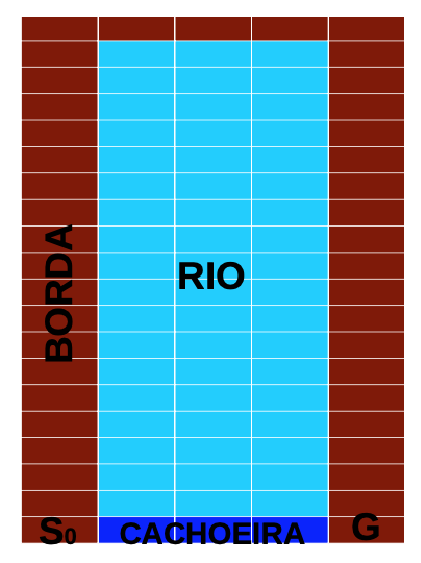
\includegraphics[width=0.9\columnwidth]{river-traversal}
    \caption{Estrutura do domínio Travessia de Rio}
    \label{fig:river-traversal-scheme}
\end{figure}

Este domínio possui 3 tamanhos de grid: um pequeno ($5 \times 25$, 125 estados), um médio ($20 \times 100$, 2000 estados) e um grande ($50 \times 250$, 12500 estados).

Os experimentos foram executados na plataforma Google Colab com o Python\footnote{Localizado em https://colab.research.google.com/drive/1KVVhy5Zi9TlpmxSn14I9H6K49K568GlY}, na época com 2 CPUs de 2.2 GHz e 13GB de memória. As implementações dos algoritmos estão disponíveis no Github\footnote{Localizado em https://github.com/danielbdias/automated-planning-and-reinforcement-learning-studies}.

A menos que o experimento diga o contrário, o resíduo máximo considerado será $ \epsilon = 0.0001 $ e o fator de desconto será de $\gamma = 0.9$.

\subsection{Experimento 1 - Convergência}

Neste experimento foi utilizado o tamanho de grid pequeno, onde os algoritmos foram executados 10 vezes e os valores médios de tempo, iterações (ou trials) e Bellman Backups foi medido. Como critério de parada para o RTDP foram assumidos 100 trials.

\begin{table}[ht]
    \caption{Métricas médias dos algoritmos}
    \label{table:exp1-mean-values}
    \begin{tabular}{llll}
        \toprule
        {}                  &      IV &    RTDP &    LRTDP \\
        \midrule
        Tempo (em segundos) & 9.38165 &  6.6939 &  5.53093 \\
        Iterações / Trials  &      33 &     100 &     42.1 \\
        Bellman Backups     &    4125 &  1423.1 &   1070.7 \\
        \bottomrule
    \end{tabular}
\end{table}

Conforme podemos ver na Tabela \ref{table:exp1-mean-values}, o algoritmo que tem a melhor performance média foi o LRTDP, executando em média 42 trials para convergir,

\begin{figure}[t]
    \centering
    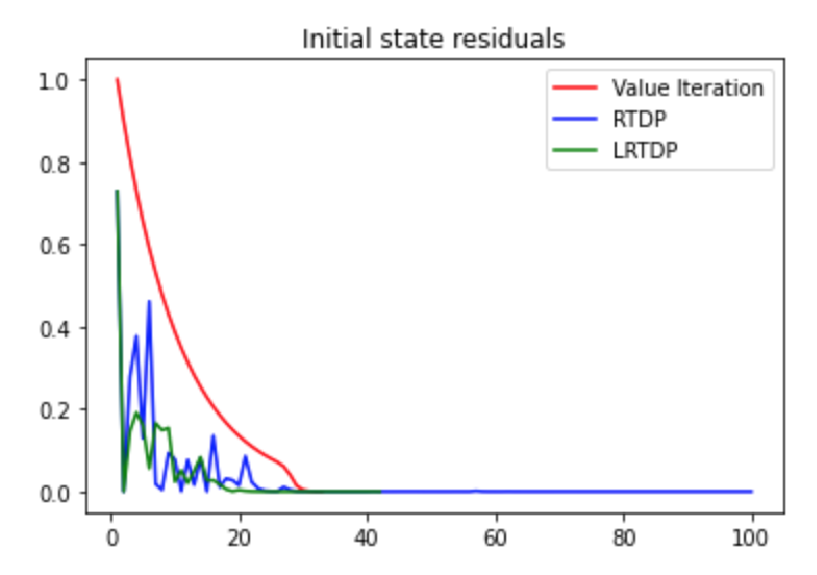
\includegraphics[width=0.9\columnwidth]{initial-state-convergency}
    \caption{Convergência do estado inicial}
    \label{fig:initial-state-convergency}
\end{figure}

%% montar mapa de calor

\subsection{Experimento 2 - Performance}

% experimento 2 comparar performances com o crescimento dos estados

\subsection{Experimento 3 - Alteração dos estados iniciais}

% experimento 3 alteração de estados iniciais

\section{Conclusão}
discuta os resultados

\bibliography{references.bib}
\bibliographystyle{aaai}

\end{document}
